\begin{surferIntroPage}{Erste Schritte mit dem SURFER}
Dieses Programm hei�t SURFER. Wenn man das Wort h�rt, denkt man an Wellen, Wasser und Sonne. Doch der Name stammt vom englischen Wort {\it surface}. Das bedeutet Fl�che.\\
Mithilfe des SURFERS k�nnen Fl�chen, genauer gesagt algebraische Fl�chen, dargestellt werden. Was algebraische Fl�chen sind und wie das Programm funktioniert, erfahren Sie hier in dieser Einf�hrung. Tippen Sie rechts auf eine der Fl�chen, um ein Kapitel auszuw�hlen. \\
Der SURFER geh�rt zur Wanderausstellung IMAGINARY. Sie wurde zum Jahr der Mathematik 2008 ins Leben gerufen. Hinter dieser Ausstellung steht das weltber�hmte Mathematische Forschungsinstitut Oberwolfach im Schwarzwald. Im Institut werden jede Woche Tagungen zu aktueller mathematischer Forschung abgehalten. Diese sind sehr wichtig, damit sich Wissenschaftlerinnen und Wissenschaftler aus der ganzen Welt �ber ihre Forschungsergebnisse austauschen k�nnen. \\
\vspace{0.2cm} \hspace{3.5cm}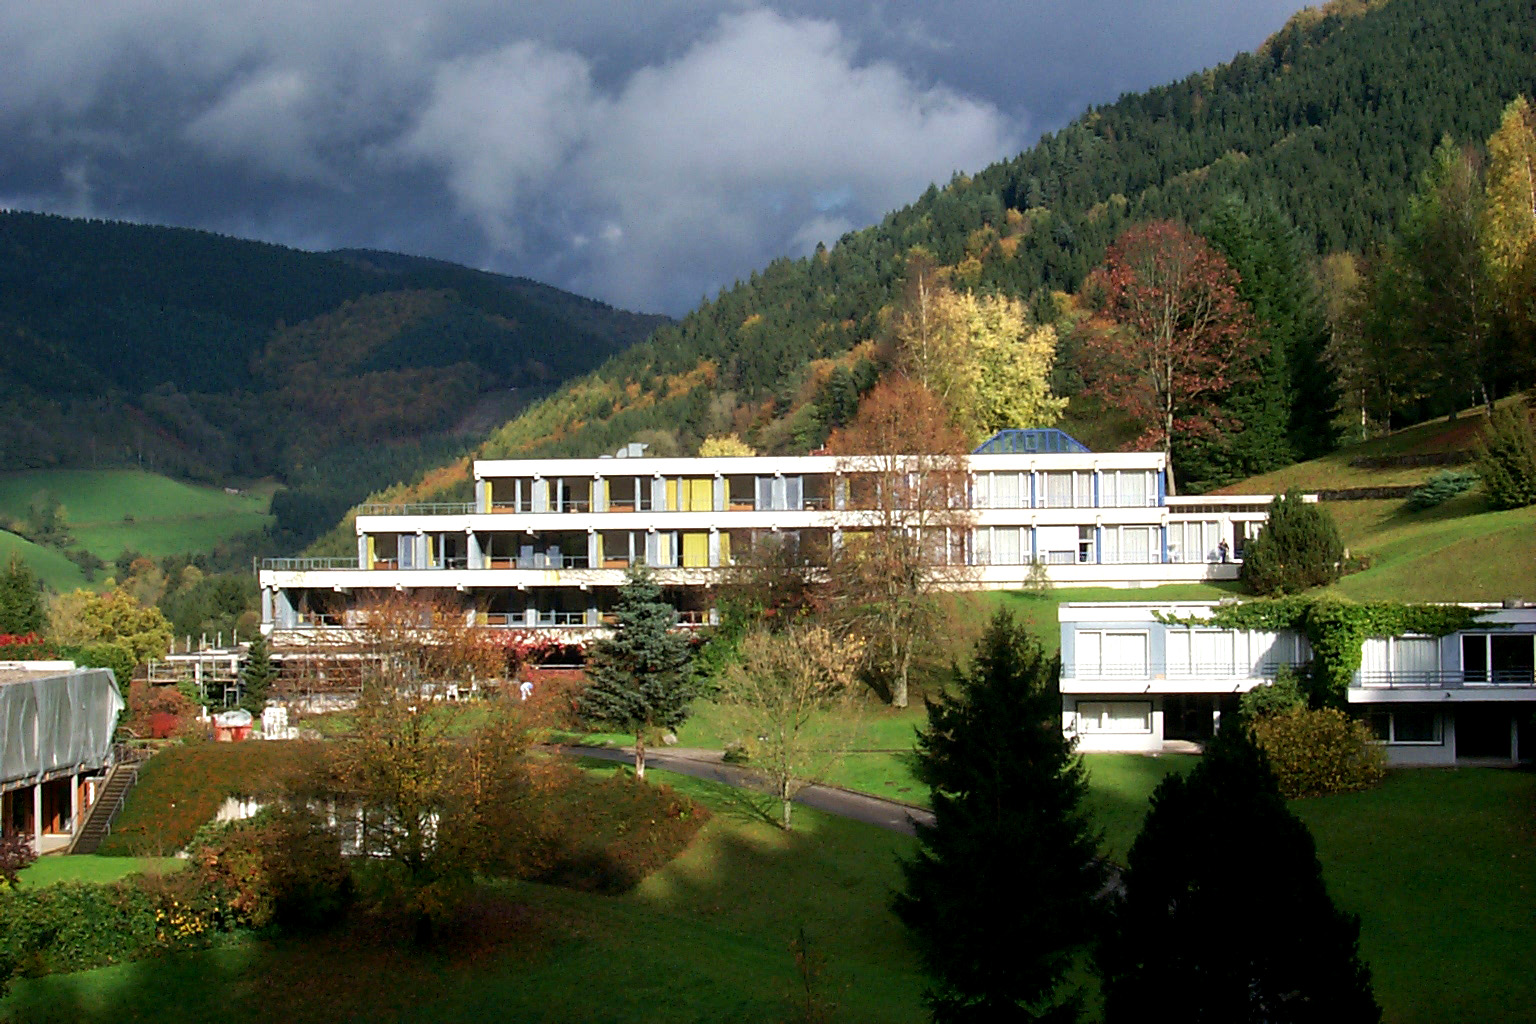
\includegraphics[width=3cm]{./../../common/images/photo_mfo.jpg}\\
Das Programm SURFER ist kostenlos auf unserer Homepage erh�ltlich: \\
\begin{centering}
www.imaginary-exhibition.com\\
\end{centering}
 \vspace{0.2cm}
Sie k�nnen rechts die mathematischen Einf�hrungen ausw�hlen, die mit der Zitrus-Fl�che beginnen. Links k�nnen Sie auf eine andere Galerie springen, z.B. die Galerie der phantasievollen Fl�chen.
\end{surferIntroPage}